% Option Pricing with Monte Carlo — DRP Poster, FSU Department of Mathematics, Spring 2025
% Author: Ibraheem Saqib Ellahi  Mentor: Pervez Ali
% 48in x 36in landscape, three columns, beamerposter.
\documentclass[final]{beamer}
\usepackage[orientation=landscape,size=custom,width=121.92,height=91.44,scale=1.6]{beamerposter}
\usepackage[T1]{fontenc}
\usepackage{lmodern}
\usepackage{amsmath,amssymb}
\usepackage{xcolor}
\usepackage{graphicx}
\usepackage{ragged2e}

% ---- FSU palette ----
\definecolor{fsugarnet}{HTML}{782F40}
\definecolor{fsugold}{HTML}{CEB888}
\definecolor{fsugrey}{HTML}{555555}

\usetheme{default}
\usecolortheme{default}
\setbeamertemplate{navigation symbols}{}

% ---- Block styling: garnet title band, gold rule, white body ----
\setbeamercolor{block title}{fg=white,bg=fsugarnet}
\setbeamercolor{block body}{fg=black,bg=white}
\setbeamerfont{block title}{series=\bfseries,size=\LARGE}
\setbeamertemplate{block begin}{
  \begin{beamercolorbox}[colsep*=1ex,rounded=false,center]{block title}
    \vskip0.2ex\usebeamerfont{block title}\insertblocktitle\vskip0.2ex
  \end{beamercolorbox}
  {\color{fsugold}\rule{\textwidth}{5pt}}\vskip-1pt
  \usebeamerfont{block body}
  \begin{beamercolorbox}[colsep*=1ex,vmode]{block body}
    \vskip0.8ex\justifying
}
\setbeamertemplate{block end}{
  \vskip0.8ex\end{beamercolorbox}\vskip1.0cm
}

\setlength{\parindent}{0em}
\setlength{\parskip}{0.6em}

% Extra breathing room between display equations and the surrounding text
\makeatletter
\g@addto@macro\normalsize{%
  \setlength\abovedisplayskip{16pt}%
  \setlength\belowdisplayskip{16pt}%
  \setlength\abovedisplayshortskip{12pt}%
  \setlength\belowdisplayshortskip{12pt}%
}
\makeatother

\begin{document}
\begin{frame}[t]

% ================= HEADER =================
\vskip0.5cm
\begin{columns}[c]
  \begin{column}{0.10\paperwidth}
    \centering
\includegraphics[width=0.82\textwidth]{../figures/logo.png}
  \end{column}
  \begin{column}{0.70\paperwidth}
    \centering
    {\fontsize{88}{96}\selectfont \color{fsugarnet}\bfseries Option Pricing with Monte Carlo}\\[0.7cm]
    {\fontsize{44}{50}\selectfont \underline{Ibraheem Saqib Ellahi}}\\[0.35cm]
    {\fontsize{36}{42}\selectfont \itshape Pervez Ali}\\[0.35cm]
    {\fontsize{36}{42}\selectfont \itshape Florida State University, Department of Mathematics}
  \end{column}
  \begin{column}{0.10\paperwidth}
    \centering
\includegraphics[width=0.82\textwidth]{../figures/logo.png}
  \end{column}
\end{columns}
\vskip0.6cm
{\centering\color{fsugarnet}\rule{\textwidth}{8pt}\par}
\vskip1.4cm

% ================= COLUMNS =================
\begin{columns}[t]

% -------- COLUMN 1: Abstract + Black-Scholes Equation --------
\begin{column}{0.30\paperwidth}

\begin{block}{Abstract}
The Black-Scholes Model was the first widely used method to calculate the theoretical value of an option contract. It derives the price of a European-style call option from an assumption of randomness, as seen in Brownian Motion. I studied the model under the guidance of a graduate student, using probability theory, stochastic calculus, and differential equations.

I then used Python to compare actual (Black-Scholes) and derived (Monte-Carlo) option prices, and plotted graphs to visualize the convergence of Monte-Carlo prices to the actual price and how option prices respond to different variables.
\end{block}

\begin{block}{Black-Scholes Equation}
We assume that the stock price follows the Stochastic DE:
\[ dS_t = \mu S_t\,dt + \sigma S_t\,dW_t \]
By Ito's Lemma:
\[ df = \left(\frac{\partial f}{\partial S}\mu S + \frac{\partial f}{\partial t} + \frac{1}{2}\frac{\partial^2 f}{\partial S^2}\sigma^2 S^2\right)dt + \frac{\partial f}{\partial S}\sigma S\,dW_t \]
For the portfolio $\Pi$ of $-1$ option and $\partial f/\partial S$ shares:
\[ \Delta\Pi = -\Delta f + \frac{\partial f}{\partial S}\Delta S \]
This portfolio is riskless, so it must earn the risk-free rate:
\[ \Delta\Pi = r\Pi\Delta t \]
Combining the two:
\[ -\left[\frac{\partial f}{\partial t} + \frac{1}{2}\sigma^2 S^2 \frac{\partial^2 f}{\partial S^2}\right]\Delta t = r\left[-f + \frac{\partial f}{\partial S}S\right]\Delta t \]
which implies the Black-Scholes partial differential equation:
\[ \frac{\partial f}{\partial t} + rS\frac{\partial f}{\partial S} + \frac{1}{2}\sigma^2 S^2\frac{\partial^2 f}{\partial S^2} = rf \]

where $S$ is the current stock price, $K$ the strike price, $f$ the price of an option depending on $S$ and $t$, $t$ the time to expiration, $r$ the risk-free rate of interest, $\sigma$ the rate of volatility, and $\Pi$ the value of the portfolio.
\end{block}

\end{column}

% -------- COLUMN 2: Graphs --------
\begin{column}{0.30\paperwidth}

\begin{block}{Graphs}
\centering
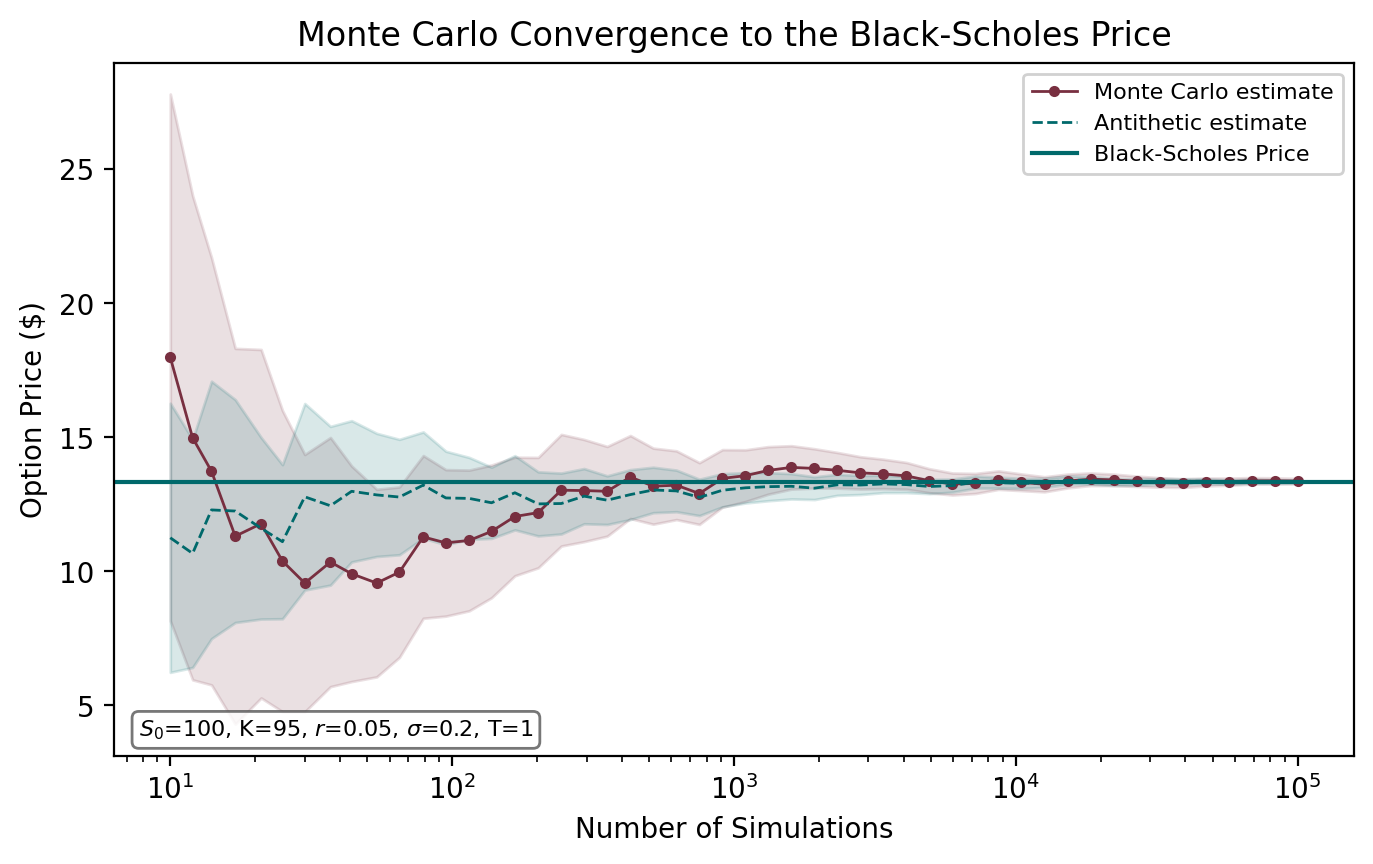
\includegraphics[width=0.78\textwidth]{../figures/convergence.png}\\[0.1cm]
{\justifying Monte-Carlo estimates converge to the Black-Scholes price as simulations grow; antithetic sampling gives a tighter confidence band.\par}\vskip0.5cm
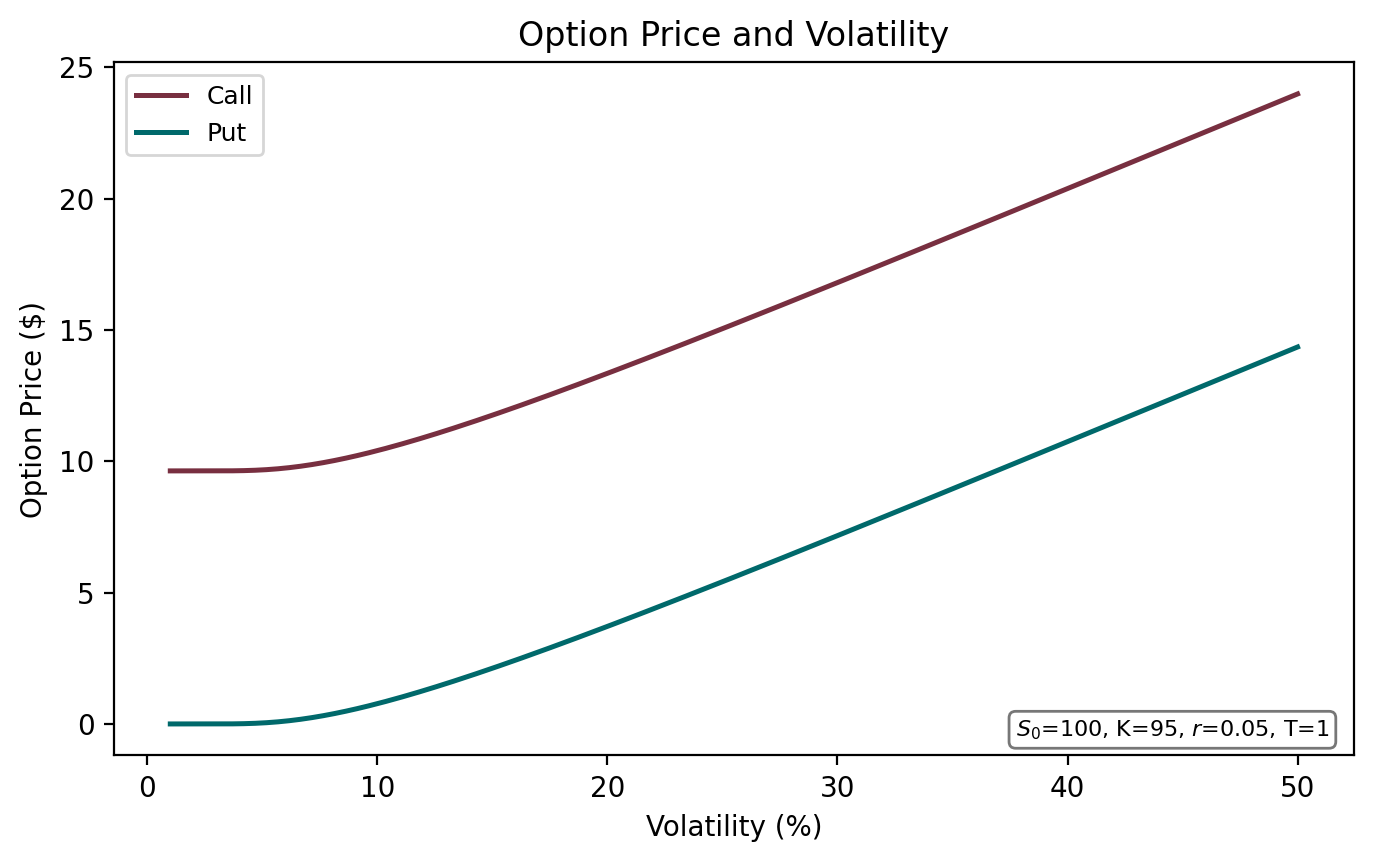
\includegraphics[width=0.78\textwidth]{../figures/price_vs_volatility.png}\\[0.1cm]
{\justifying Higher volatility raises option prices: more volatility means more upside potential.\par}\vskip0.5cm
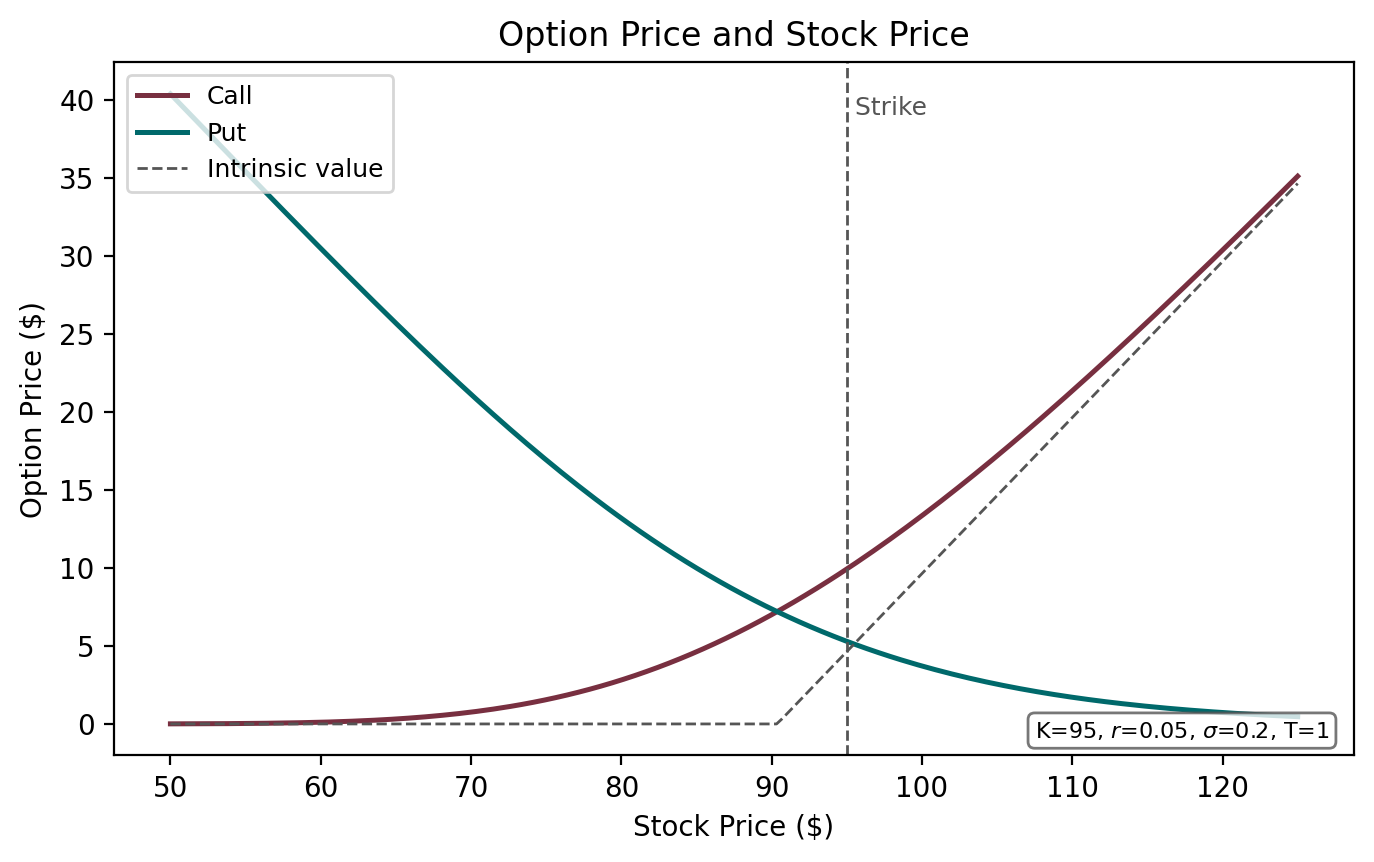
\includegraphics[width=0.78\textwidth]{../figures/price_vs_stock_price.png}\\[0.1cm]
{\justifying The call price rises with the stock price above the strike and flattens toward zero below it.\par}
\end{block}

\end{column}

% -------- COLUMN 3: Modelling & Motivations + Question + Conclusion --------
\begin{column}{0.30\paperwidth}

\begin{block}{Modelling \& Motivations}
The Black-Scholes PDE can be solved to give the call price $C$ and put price $P$:
\[ C = S_0 N(d_1) - K e^{-rT} N(d_2) \]
\[ P = K e^{-rT} N(-d_2) - S_0 N(-d_1) \]

A call option gives the holder a right, but not an obligation, to buy a stock at a predetermined price on a later date; a put option gives the right to sell. Options give exposure to a stock with a smaller investment, but are generally much riskier.

These models let traders control the risks of options trading and enabled the development of the derivatives market. Their strong assumptions do not always hold, so prices will not always match the market, but they still convey real information about how options behave.

I performed the calculations and plotted the graphs in Python using the NumPy, SciPy, and Matplotlib libraries.
\end{block}

\begin{block}{Question}
What do you think the option price will be with these variables?

\begin{center}
\renewcommand{\arraystretch}{1.2}
\begin{tabular}{l r}
\hline
Current stock price & \$100 \\
Strike price & \$95 \\
Time to expiration & 1 year \\
Risk-free interest rate & 5\% \\
Volatility & 20\% \\
\hline
\end{tabular}
\end{center}
\end{block}

\begin{block}{Conclusion}
Adjusting different variables in the Black-Scholes Model and Monte Carlo calculations results in a deeper understanding of how option prices vary and has important real world implications.

I would like to thank Pervez Ali for being a wonderful mentor for this project.
\end{block}

\end{column}

\end{columns}
\end{frame}
\end{document}
